\documentclass[simplex.tex]{subfiles}
% NO NEED TO INPUT PREAMBLES HERE
% packages are inherited; you can compile this on its own
\begin{document}
\subsection{Robust Law of Large Graphs}

In order to see a bias-variance tradeoff phenomenon with respect to the parameter $q$ in the ML$q$E estimator, we change our simulation setting as following:
We consider the 2-block SBM with respect to the exponential distributions parameterized by
\begin{equation*}
B = \begin{bmatrix}
4 & 2 \\
2 & 7
\end{bmatrix}
,\qquad \rho = \begin{bmatrix}
0.5 & 0.5
\end{bmatrix}.
\end{equation*}
And let the contamination also be a 2-block SBM with the same structure parameterized by
\begin{equation*}
B^{\prime} = \begin{bmatrix}
9 & 6 \\
6 & 13
\end{bmatrix}
,\qquad \rho = \begin{bmatrix}
0.5 & 0.5
\end{bmatrix}.
\end{equation*}

Figure~\ref{fig:q} shows the mean squared error in average by varying the parameter $q$ in ML$q$E with fixed $n = 100$, $m = 20$ and $\epsilon = 0.1$ based on 1000 Monte Carlo replicates. Different types of lines represent the simulated MSE associated with four different estimators. From the figure, we can see that the ASE procedure takes advantage of the graph structure and improves the performance of the corresponding estimators independent of the selection of $q$. Moreover, within a proper range of $q$, the ML$q$E wins the bias-variance tradeoff and shows the robustness property compare to the MLE. And as $q$ goes to 1, ML$q$E goes to the MLE as expected.

\begin{figure}[!htb]
\centering
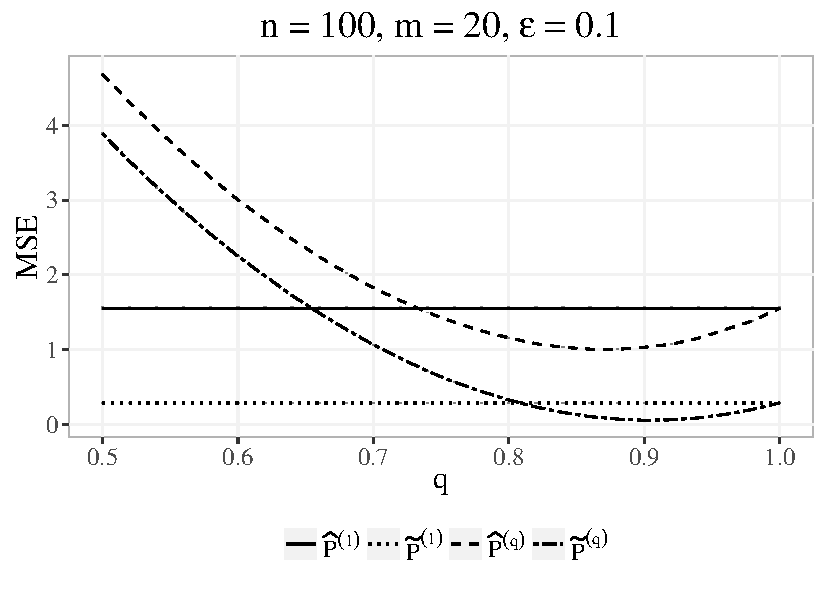
\includegraphics[width=0.7\textwidth]{../../figs/sim_q.pdf}
\caption{Mean squared error in average by varying the parameter $q$ in ML$q$E with fixed $n = 100$, $m = 20$ and $\epsilon = 0.1$ based on 1000 Monte Carlo replicates. Different types of lines represent the simulated MSE associated with four different estimators.
1. ASE procedure takes advantage of the graph structure and improves the performance of the corresponding estimators independent of the selection of $q$;
2. Within a proper range of $q$, ML$q$E wins the bias-variance tradeoff and shows the robustness property compare to the MLE. Also as $q$ goes to 1, ML$q$E goes to the MLE as expected.}
\label{fig:q}
\end{figure}

\clearpage
\end{document}
